\section{Results}
\label{sec:results}
\subsection{Decision Latency and Semantic Accuracy}
% Generated by scripts/plot_section_paper_results.py.
\begin{figure*}[!t]
\centering
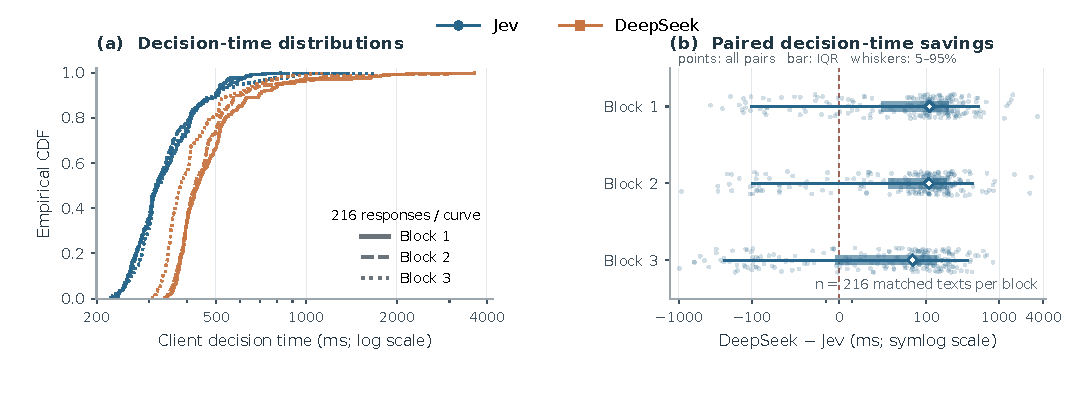
\includegraphics[width=\textwidth]{figures/decision-latency.pdf}
\caption{Study A decision latency on the same 216 texts per model and
consecutive block. (a) Full client response-time cumulative distribution
functions (CDFs) on a logarithmic time
axis. (b) All paired DeepSeek-minus-Jev differences: points, interquartile
bars, nearest-rank 5th--95th percentile whiskers, and median diamonds. The
symmetric-log axis is linear within $\pm50$\,ms. The ranges describe request
variation, not confidence intervals; texts recur across blocks.}
\label{fig:decision-latency}
\end{figure*}

Table~\ref{tab:quality} reports all three Study A blocks. Jev's median full
client decision time is 314.7--320.7\,ms, compared with DeepSeek's
381.4--434.7\,ms. The corresponding reductions are 26.5\%, 26.1\%, and
15.9\% in block order. Empirical p95 latency is also lower in each block,
by 36.7\%, 33.0\%, and 9.1\%, respectively. Jev's advantage varies across
the three blocks. Figure~\ref{fig:decision-latency} shows the full distributions
and their paired request-level differences.

\begin{table}[t]
\caption{Study A: exact four-field correctness and client decision latency.
Each row contains 216 requests; the same texts recur across blocks.}
\label{tab:quality}
\centering
% Generated by ../scripts/export_paper_draft_assets.py; do not hand-edit values.
\begin{tabular}{@{}clrrr@{}}
\toprule
Block & Backend & Correct & Median (ms) & p95 (ms) \\
\midrule
1 & Jev & 214/216 & 319.5 & 529.3 \\
1 & DeepSeek & 216/216 & 434.7 & 835.9 \\
2 & Jev & 213/216 & 314.7 & 557.8 \\
2 & DeepSeek & 215/216 & 425.9 & 833.2 \\
3 & Jev & 212/216 & 320.7 & 624.2 \\
3 & DeepSeek & 216/216 & 381.4 & 686.9 \\
\bottomrule
\end{tabular}

\end{table}

% Generated by scripts/plot_section_paper_results.py.
\begin{figure}[!tb]
\centering
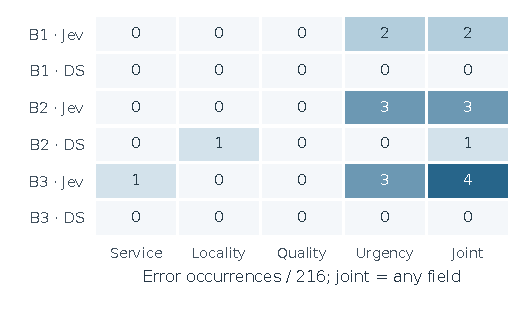
\includegraphics[width=\columnwidth]{figures/semantic-errors.pdf}
\caption{Study A semantic-error profile, with 216 responses per row.
Joint counts indicate an error in any field; B1--B3 are consecutive blocks
on reused texts, and DS denotes DeepSeek.}
\label{fig:semantic-errors}
\end{figure}


Both hosted APIs return schema-valid fields throughout Study A. DeepSeek
is more accurate on the strict semantic endpoint: it gets
216, 215, and 216 requests correct, versus Jev's 214, 213, and 212. Jev's
nine error occurrences span five distinct texts. Eight occurrences replace
unspecified urgency with normal urgency; the ninth maps an unsupported
recorded-speech translation request to OCR. This synthetic description
combines an unsupported translation intent with an image-transfer permission
clause. DeepSeek's single error replaces remote permission with unspecified
locality. Lower Jev decision latency therefore accompanies lower exact
semantic accuracy. Figure~\ref{fig:semantic-errors} resolves the errors by
field and block.

Operational equivalence explains why this semantic gap need not reduce
completion. Normal and unspecified urgency both map to ordinary
priority in this scheduler, so that field mismatch can leave execution
unchanged. In contrast, interpreting translation as OCR can dispatch the
wrong service. The latter text was not selected into Study A's execution
traces, so its effect is absent from the modeled completion results.

\subsection{Completion with Modeled Execution}
% Generated by scripts/plot_section_paper_results.py.
\begin{figure}[!tb]
\centering
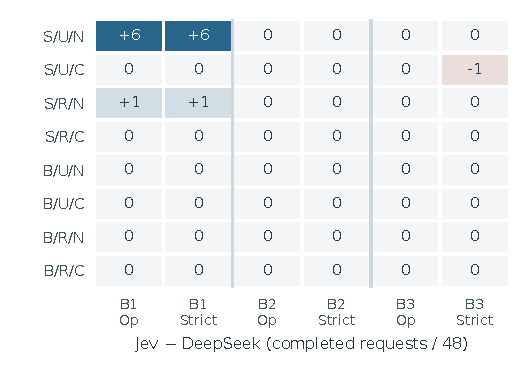
\includegraphics[width=\columnwidth]{figures/modeled-completion.pdf}
\caption{Study A completion differences across all 24 paired
conditions. Each cell is Jev minus DeepSeek, out of 48 arrivals. Op checks
operational requirements; Strict also requires exact field equality.
B1--B3 identify consecutive blocks. S/B denote steady/bursty arrivals, U/R changing/repeated text, and N/C cache off/on.}
\label{fig:modeled-completion}
\end{figure}

Across Study A's 24 paired conditions, Jev and DeepSeek have equal operational
completion counts in 22, and Jev has higher counts in two
(Fig.~\ref{fig:modeled-completion}). Summing the fixed matrix yields 884/884 supported
arrivals completed by Jev and 877/884 by DeepSeek. Each backend also receives
268 unsupported arrivals, which remain separate from execution successes.
The strict companion endpoint gives 21 ties, two conditions higher for Jev,
and one lower. In the latter condition, the loss is an unspecified-to-normal
urgency mismatch with the same executed priority, in a condition with no
cache hits.

% Generated by scripts/plot_section_paper_results.py.
\begin{figure*}[!t]
\centering
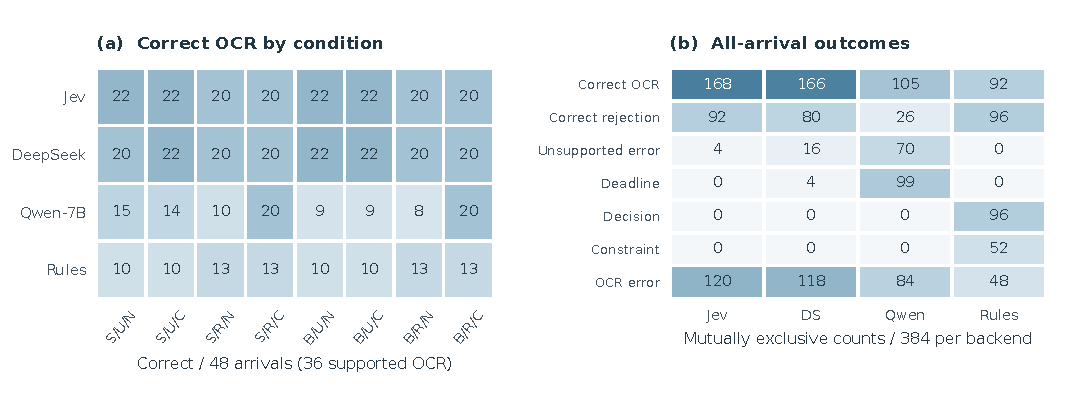
\includegraphics[width=\textwidth]{figures/ocr-outcomes.pdf}
\caption{Study B real-service outcomes, one run per condition and backend.
(a) Correct, on-time OCR completions in all 32 arms, each with 48 arrivals
and 36 supported requests. (b) Mutually exclusive outcomes among all 384
arrivals per backend; DS denotes DeepSeek. S/B denote steady/bursty arrivals, U/R changing/repeated text, and N/C cache off/on.}
\label{fig:ocr-outcomes}
\end{figure*}


Both operational gains occur in the first block without caching. In its
steady-changing condition, four DeepSeek calls take approximately
5.44--5.81\,s, and four additional arrivals expire while waiting. Six of
these eight failures are supported requests, yielding 36 Jev completions
versus 30 DeepSeek completions. In steady-repeated traffic, one supported
DeepSeek request lacks enough execution slack after waiting, yielding 41
versus 40 completions. These trajectories show how delayed decisions can
propagate into queueing and missed deadlines.

\subsection{Correct Completion in the Real OCR Service}

Table~\ref{tab:outcomes} aggregates the same eight conditions per backend.
Jev completes 168/288 supported requests correctly and on time (58.3\%),
versus 166/288 for DeepSeek (57.6\%). Qwen and rules complete 105/288 (36.5\%)
and 92/288 (31.9\%), respectively. Figure~\ref{fig:ocr-outcomes} retains all 384
arrivals per backend, including the 96 unsupported requests.

\begin{table}[t]
\caption{Study B: aggregate outcomes over eight conditions per backend.
Completed OCR and correctly rejected requests have different denominators.
False admissions count unsupported requests actually dispatched to OCR.}
\label{tab:outcomes}
\centering
% Generated by ../scripts/export_paper_draft_assets.py; do not hand-edit values.
\begin{tabular}{@{}lrrr@{}}
\toprule
Backend & Correct OCR & Correct rejection & False admit \\
\midrule
Jev & 168/288 & 92/96 & 4 \\
DeepSeek & 166/288 & 80/96 & 13 \\
Qwen2.5-7B & 105/288 & 26/96 & 4 \\
Rules & 92/288 & 96/96 & 0 \\
\bottomrule
\end{tabular}

\end{table}

Jev matches DeepSeek's correct-completion count in seven conditions and
exceeds it by two in one (Table~\ref{tab:paired}). Service-output errors
remain substantial: the outcome breakdown
attributes 120 Jev arrivals and 118 DeepSeek arrivals to OCR content or
execution failure, after preceding failure categories have been excluded.
Checking the returned text exposes these failures even when the decision
and service calls themselves succeed.

Among unsupported requests, Jev correctly rejects
92/96 and dispatches four unsupported requests to OCR. All four are repeated
occurrences of one translation intent across conditions. DeepSeek correctly
rejects 80/96, with 13 actual false
admissions; the remaining three mishandled unsupported requests do not result
in an OCR dispatch. Rules reject all 96 unsupported requests, but also lose
supported jobs through interpretation and execution-constraint failures.
No forbidden off-site image bytes are observed for any backend in these
runs, which include 22 remote executions for Jev and 30 for DeepSeek.

\begin{table*}[!t]
\caption{Study B: all Jev--DeepSeek paired conditions. Each condition has 48
arrivals, of which 36 require OCR. Completion counts retain all failures;
latencies use only the $N$ requests completed correctly by both backends.
Positive paired saving means faster completion with Jev.}
\label{tab:paired}
\centering
% Generated by ../scripts/export_paper_draft_assets.py; do not hand-edit values.
\begin{tabular}{@{}lllrrrrrr@{}}
\toprule
 & & & \multicolumn{2}{c}{Correct completions} & & \multicolumn{2}{c}{Median full time (ms)} & Median paired \\
\cmidrule(lr){4-5}\cmidrule(lr){7-8}
Load & Description & Cache & Jev & DeepSeek & $N$ & Jev & DeepSeek & saving (ms) \\
\midrule
Steady & Changing & Off & 22 & 20 & 20 & 410.4 & 538.6 & 135.69 \\
Steady & Changing & On & 22 & 22 & 22 & 418.3 & 483.1 & 84.93 \\
Steady & Repeated & Off & 20 & 20 & 20 & 436.4 & 490.8 & 70.63 \\
Steady & Repeated & On & 20 & 20 & 20 & 110.9 & 112.4 & -0.37 \\
Bursty & Changing & Off & 22 & 22 & 22 & 438.7 & 587.6 & 101.14 \\
Bursty & Changing & On & 22 & 22 & 22 & 478.2 & 515.2 & 74.43 \\
Bursty & Repeated & Off & 20 & 20 & 20 & 436.3 & 555.5 & 125.86 \\
Bursty & Repeated & On & 20 & 20 & 20 & 106.2 & 109.0 & -0.49 \\
\bottomrule
\end{tabular}

\end{table*}

\subsection{End-to-End Latency and the Cache Boundary}
% Generated by scripts/plot_section_paper_results.py.
\begin{figure}[!tb]
\centering
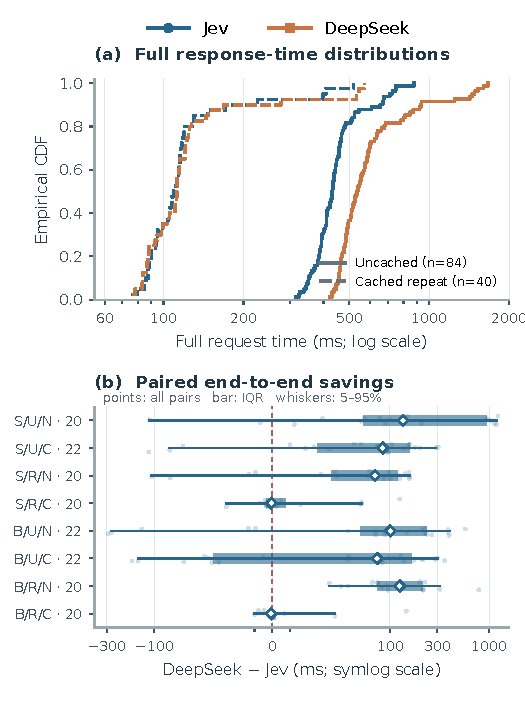
\includegraphics[width=\columnwidth]{figures/ocr-latency.pdf}
\caption{Study B latency on requests completed correctly by both
Jev and DeepSeek. (a) Descriptive pooled CDFs; sample size $n$ is 84 per model
for the four uncached conditions and 40 for the two repeated-text cached
conditions. Changing-text cached arms are excluded from this panel.
(b) Every paired difference in all eight conditions; row suffixes give $n$.
Bars show the interquartile range, whiskers the nearest-rank 5th--95th
percentiles, and diamonds the median. The symmetric-log axis is linear
within $\pm50$\,ms. Ranges are descriptive, not confidence intervals.
S/B denote steady/bursty arrivals, U/R changing/repeated text, and N/C cache off/on.}
\label{fig:ocr-latency}
\end{figure}

On the common-success subset, Jev reduces median full request latency by
11.1--25.3\% in the four cache-disabled conditions. These comparisons contain
20 or 22 paired successful requests each. Median per-request savings range
from 70.6 to 135.7\,ms (Table~\ref{tab:paired}). These durations include
image transfer, worker queueing, OCR execution, and response delivery.

% Generated by scripts/plot_section_paper_results.py.
\begin{figure}[!tb]
\centering
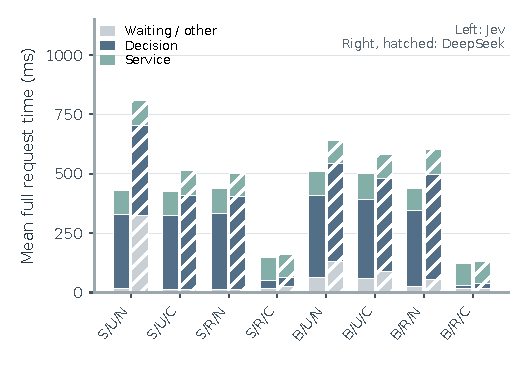
\includegraphics[width=\columnwidth]{figures/ocr-time-components.pdf}
\caption{Study B mean time composition on each condition's
common-success subset. The service component includes transfer and OCR; the residual
includes queueing and controller handling. Left bars are Jev; right,
hatched bars are DeepSeek. Components sum to the arithmetic mean, not the
median. S/B denote steady/bursty arrivals, U/R changing/repeated text, and N/C cache off/on.}
\label{fig:ocr-time-components}
\end{figure}


Figure~\ref{fig:ocr-latency}b retains every paired latency difference, including
requests on which DeepSeek is faster. Figure~\ref{fig:ocr-time-components}
decomposes mean full time on the same successful subsets. Its service component includes
image transfer and OCR; the remaining time includes controller handling and
queueing.

Caching changes the result when descriptions repeat. With caching enabled,
the steady-repeated medians are 110.9\,ms for Jev and 112.4\,ms for DeepSeek;
the bursty-repeated medians are 106.2 and 109.0\,ms. Yet the median paired
savings are $-0.37$ and $-0.49$\,ms, respectively. The small opposite signs
arise because a difference of marginal medians is not a median of paired
differences. Neither comparison supports a material latency advantage after
the reusable decisions are cached. Figure~\ref{fig:ocr-latency}a also contrasts
the uncached and repeated-text cached response-time distributions. Changing-text conditions have no exact
cache hits; differences between their cache-on and cache-off arms reflect
separate executions, not a benefit from cache lookup.

Qwen has
105 correct completions in the full matrix and 99 arrivals classified as
deadline or infeasibility failures. Its conditional median model-call time
is 1.408\,s, consuming a substantial part of the request budget before
service execution.
The called request subsets differ across backends because of cache hits and
expiry, so this conditional median is diagnostic rather than a paired
model-speed benchmark. With repeated-text caching, Qwen reaches 20 correct
completions in both load conditions, matching the hosted backends there.

\subsection{Billed API Cost}
% Generated by scripts/plot_section_paper_results.py.
\begin{figure}[!tb]
\centering
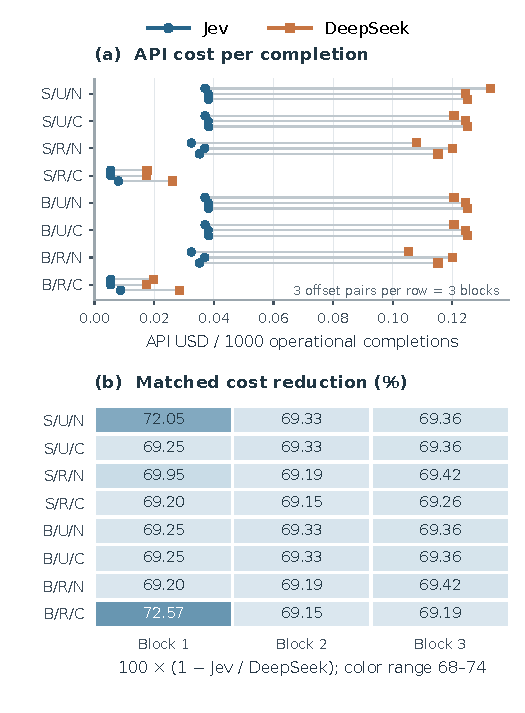
\includegraphics[width=\columnwidth]{figures/modeled-api-cost.pdf}
\caption{Study A billed API cost per modeled operational completion.
(a) Absolute fees, scaled to 1000 completions; top-to-bottom offsets within
each row distinguish blocks 1--3. (b) Matched reductions, with color range
68--74\%. Fees include all trajectory calls and exclude warmups and
separate quality evaluation. S/B denote steady/bursty arrivals, U/R changing/repeated text, and N/C cache off/on.}
\label{fig:modeled-api-cost}
\end{figure}

Study A's API fees per operational completion are 69.15--72.57\% lower
with Jev across the 24 pairs (Fig.~\ref{fig:modeled-api-cost}). These costs
include unsuccessful requests and use observed modeled completion counts.
The absolute fees and matched reductions retain all three blocks separately.

% Generated by scripts/plot_section_paper_results.py.
\begin{figure}[!tb]
\centering
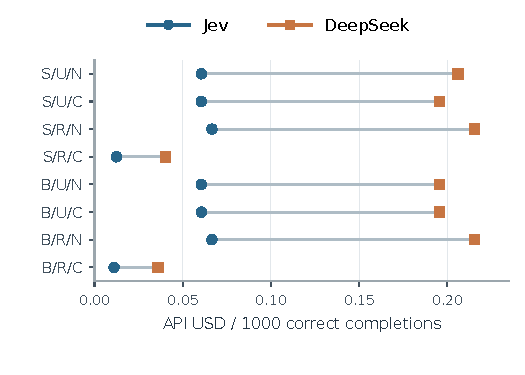
\includegraphics[width=\columnwidth]{figures/ocr-api-cost.pdf}
\caption{Study B API fees per correct OCR completion, scaled to
1000. Charges include all trajectory calls, including unsuccessful
requests, but exclude warmups, computation, network, and other operating
costs. S/B denote steady/bursty arrivals, U/R changing/repeated text, and N/C cache off/on.}
\label{fig:ocr-api-cost}
\end{figure}

Jev's API fees per correct OCR completion are 68.97--70.61\% lower over all
eight paired conditions; the cache-disabled range is 69.03--70.61\%.
Depending on the condition, the observed values scale to approximately
\$0.011--\$0.067 per 1000 correct completions for Jev, versus
\$0.036--\$0.215 for DeepSeek (Fig.~\ref{fig:ocr-api-cost}).

Caching reduces the absolute fee for both models and leaves a similar
relative API-cost gap on the remaining calls.
